\subsection{Interval estimate}
\label{sec:etas-interval}

\begin{itemize}
\item emphasise that ETAs are symmetric on the probability scale, but not (necessarily) on the arrival time scale (due to lower bound)
\item KF approach gives normal predictions, giving symmetric interval on arrival time scale also (which is probably wrong)
\end{itemize}

Deciding on a ``best'' single-value estimate of arrival time is exceedingly difficult given the amount of uncertainty involved. An alternative approach would be to provide \emph{two} estimates---a lower and upper bound---that is to say, a \emph{prediction interval}. To do so, we need to consult the following criteria:
the probability of the bus arriving outside the interval versus the width of the interval; and
the probability of the bus arriving before the lower bound versus the expected waiting time (given arrival at the lower bound).
The first point corresponds to how useful---from a commuter's point of view---the prediction is: a narrow interval is favourable, but we must balance that with covering a reasonable range of plausible values. The second point again relates to \emph{cost}, which we can most easily express as expected waiting time; there are, of course, other costs (such as being late for work), which we examine more closely in \cref{sec:etas-journey-planning}.







\begin{knitrout}\small
\definecolor{shadecolor}{rgb}{0.969, 0.969, 0.969}\color{fgcolor}\begin{figure}

{\centering 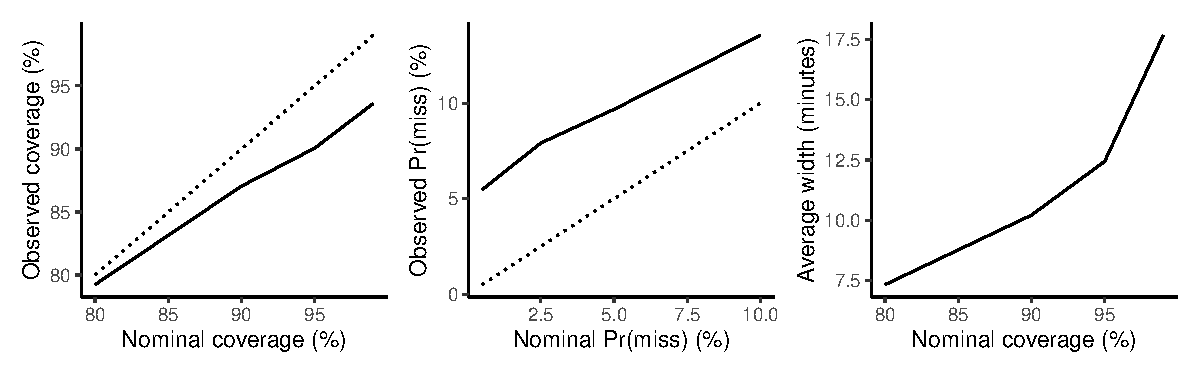
\includegraphics[width=\textwidth]{figure/eta_cis-1} 

}

\caption[ETA CIs]{ETA CIs}\label{fig:eta_cis}
\end{figure}


\end{knitrout}


The most straightforward intervals to compute are \emph{symmetric}\footnote{They are not perfectly symmetric, however, due to integer rounding}. That is, for a \mbox{$100(1-\alpha)$\%} interval we use $A_{\alpha/2}$ and $A_{1-\alpha/2} + 1$ (the plus one on the upper bound is so the upper bound is effectively rounded up). We computed intervals for $\alpha \in \{0.1, 0.05, 0.1, 0.2\}$, and for each evaluated the observed coverage, the probability that the bus arrived before the lower bound, and the average width (in minutes). The graphs in \cref{fig:eta_cis} show that for smaller values of $\alpha$ (larger coverage) the coverage probability and average width increase, which is to be expected. Similarly, the probability that the bus arrives before the lower bound (resulting in missing the bus) increases with $\alpha$.

An alternative to using symmetric intervals is to use asymmetric ones: in this scenario, the lower and upper bounds could be estimated using different criteria. For example, the lower bound might be chosen to minimise the chance of missing the bus, while the upper bound is chosen to balance excessive width while still covering as greater plausible range as possible. Again, we might also wish to vary the criteria depending on the proximity of the bus, the stop sequence, or headway. \textcolor{red}{[to do, I suppose]}
